\documentclass{article}
\usepackage[utf8]{inputenc}
\usepackage{amsmath}
\usepackage{graphicx}
\usepackage{geometry}
\usepackage{xcolor}
\geometry{a4paper, margin=1in}

\begin{document}

\begin{figure}[h]
    \centering
    % IMPORTANT: Ensure your uploaded image file is named op_amp.png
    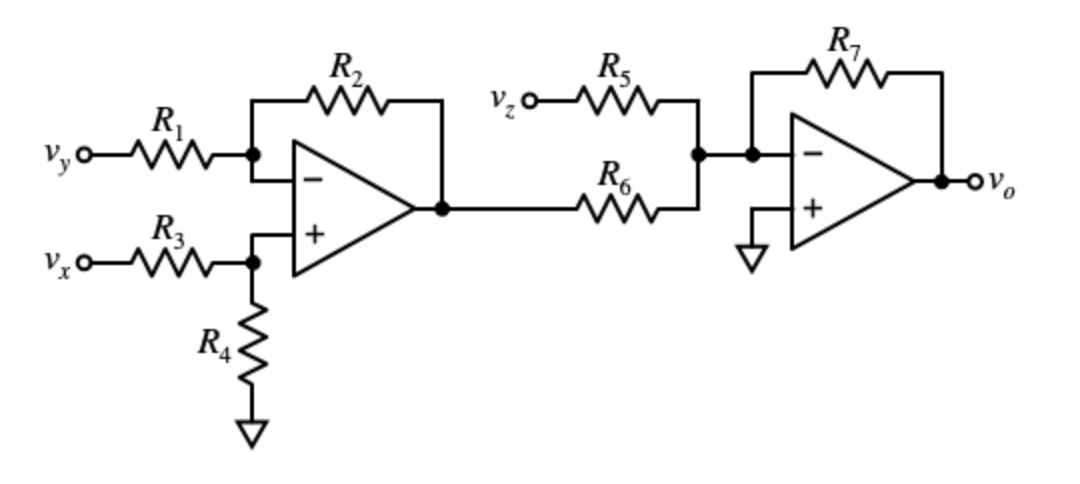
\includegraphics[width=0.7\textwidth]{op_amp.png}
    \caption{Multi-stage Op-Amp Circuit}
    \label{fig:circuit}
\end{figure}


For the circuit shown in Figure \ref{fig:circuit}, the resistor values are given as:
\begin{itemize}
    \item $R_1 = R_3 = 1 \text{ k}\Omega$
    \item $R_2 = R_4 = 1.5 \text{ k}\Omega$
    \item $R_5 = R_7 = 10 \text{ k}\Omega$
    \item $R_6 = 5 \text{ k}\Omega$
\end{itemize}

Find the expression for the output voltage $v_o$ in terms of $v_x$, $v_y$, and $v_z$.
{\color{blue} 

\subsection*{Solution}

\textbf{1. First Stage Analysis (Difference Amplifier)} \\
The first op-amp stage acts as a difference amplifier. Since the resistor pairs are matched ($R_1 = R_3$ and $R_2 = R_4$), the output $v_{o1}$ is:
\begin{equation*}
    v_{o1} = \frac{R_2}{R_1}(v_x - v_y) = \frac{1.5}{1}(v_x - v_y) = 1.5v_x - 1.5v_y
\end{equation*}

\textbf{2. Second Stage Analysis (Inverting Summing Amplifier)} \\
The second stage takes the output of the first stage ($v_{o1}$) and the input $v_z$ through $R_6$ and $R_5$ respectively. The output $v_o$ is calculated as:
\begin{equation*}
    v_o = -\left( \frac{R_7}{R_6}v_{o1} + \frac{R_7}{R_5}v_z \right)
\end{equation*}

\textbf{3. Numerical Calculation and Final Expression} \\
Calculating the gains for the second stage:
\begin{itemize}
    \item Gain for $v_{o1}$: $\frac{R_7}{R_6} = \frac{10}{5} = 2$
    \item Gain for $v_z$: $\frac{R_7}{R_5} = \frac{10}{10} = 1$
\end{itemize}

Substituting $v_{o1}$ into the equation:
\begin{align*}
    v_o &= -(2(1.5v_x - 1.5v_y) + 1 \cdot v_z) \\
    v_o &= -(3v_x - 3v_y + v_z)
\end{align*}

\subsection*{Final Answer}
The final expression for the output voltage is:
\begin{equation}
    v_o = -3v_x + 3v_y - 1v_z
\end{equation}

}
\end{document}